% REDI Operational Modes Diagram
% Shows the three modes: run, discover, sidecar
% For paper: "REDI: Automated Data Readiness for Scientific AI"

\documentclass[tikz,border=10pt]{standalone}
\usepackage{tikz}
\usetikzlibrary{shapes.geometric, arrows.meta, positioning, fit, backgrounds, calc, decorations.pathreplacing}

% Color scheme
\definecolor{rediblue}{RGB}{41, 98, 255}
\definecolor{redipurple}{RGB}{103, 58, 183}
\definecolor{redigreen}{RGB}{0, 150, 136}
\definecolor{rediorange}{RGB}{255, 152, 0}
\definecolor{redigray}{RGB}{96, 125, 139}

\begin{document}
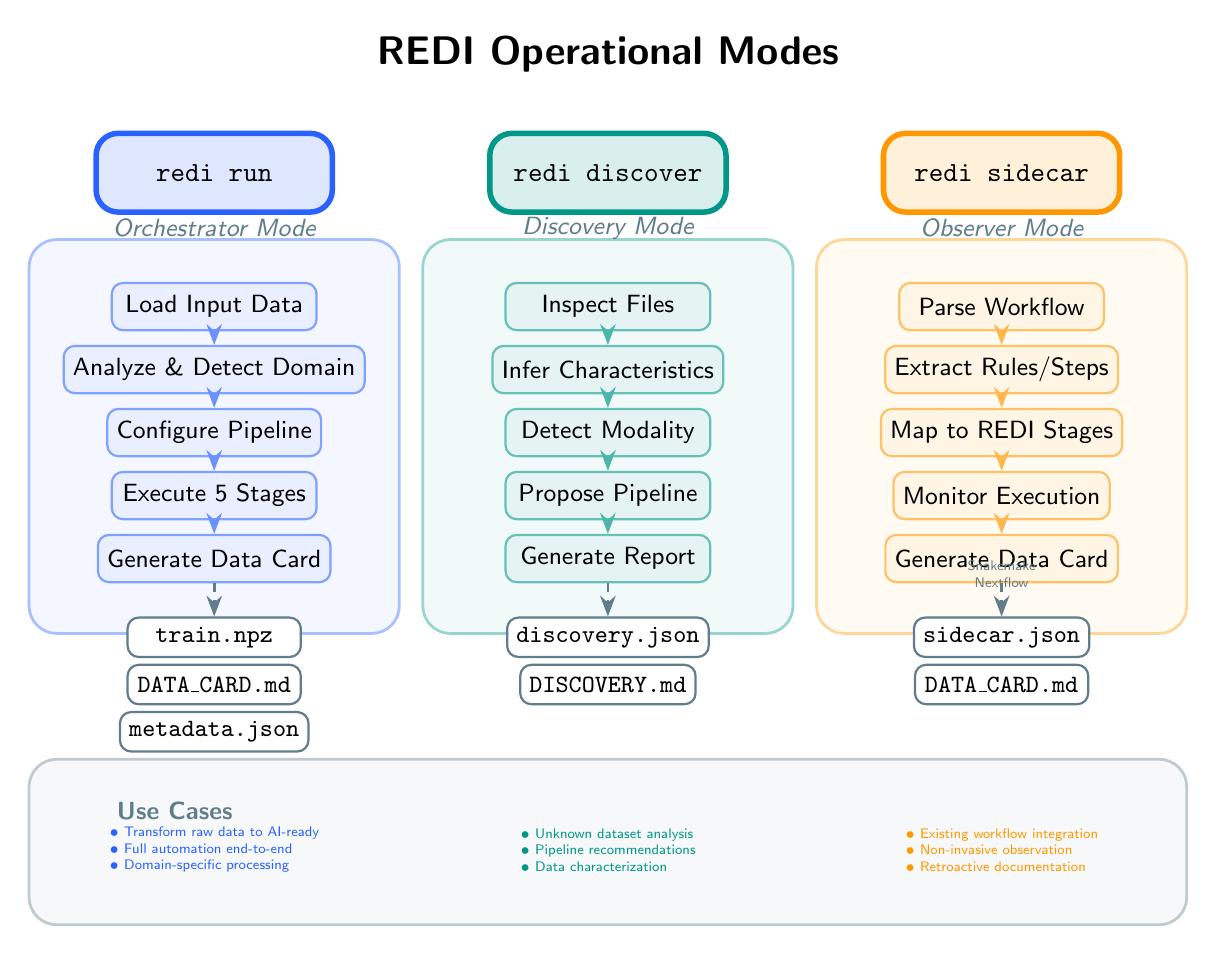
\begin{tikzpicture}[
    mode/.style={
        rectangle, rounded corners=8pt, minimum width=3cm, minimum height=1cm,
        draw=#1, line width=2pt, fill=#1!15, font=\bfseries\sffamily
    },
    step/.style={
        rectangle, rounded corners=4pt, minimum width=2.6cm, minimum height=0.6cm,
        draw=#1!60, line width=0.8pt, fill=#1!10, font=\small\sffamily
    },
    output/.style={
        rectangle, rounded corners=4pt, minimum width=2.2cm, minimum height=0.5cm,
        draw=redigray, line width=0.8pt, fill=white, font=\small\ttfamily
    },
    arrow/.style={->, >=Stealth, line width=1pt, color=redigray},
    groupbox/.style={rectangle, rounded corners=10pt, draw=#1!40, line width=1pt, fill=#1!5, inner sep=10pt}
]

% Title
\node[font=\Large\bfseries\sffamily] at (0, 8.5) {REDI Operational Modes};

% ============================================================================
% MODE 1: RUN (Orchestrator)
% ============================================================================
\node[mode=rediblue] (runmode) at (-5, 7) {\texttt{redi run}};
\node[font=\small\sffamily\itshape, text=redigray] at (-5, 6.3) {Orchestrator Mode};

\begin{scope}[on background layer]
    \node[groupbox=rediblue, fit={($ (-7, 5.8) $) ($ (-3, 1.5) $)}] {};
\end{scope}

% Run mode workflow
\node[step=rediblue] (r1) at (-5, 5.3) {Load Input Data};
\node[step=rediblue] (r2) at (-5, 4.5) {Analyze \& Detect Domain};
\node[step=rediblue] (r3) at (-5, 3.7) {Configure Pipeline};
\node[step=rediblue] (r4) at (-5, 2.9) {Execute 5 Stages};
\node[step=rediblue] (r5) at (-5, 2.1) {Generate Data Card};

\draw[arrow, color=rediblue!70] (r1) -- (r2);
\draw[arrow, color=rediblue!70] (r2) -- (r3);
\draw[arrow, color=rediblue!70] (r3) -- (r4);
\draw[arrow, color=rediblue!70] (r4) -- (r5);

% Run mode outputs
\node[output] (ro1) at (-5, 1.1) {train.npz};
\node[output] (ro2) at (-5, 0.5) {DATA\_CARD.md};
\node[output] (ro3) at (-5, -0.1) {metadata.json};

\draw[arrow, dashed] (r5.south) -- ++(0, -0.3) -- (ro1.north);

% ============================================================================
% MODE 2: DISCOVER
% ============================================================================
\node[mode=redigreen] (discovermode) at (0, 7) {\texttt{redi discover}};
\node[font=\small\sffamily\itshape, text=redigray] at (0, 6.3) {Discovery Mode};

\begin{scope}[on background layer]
    \node[groupbox=redigreen, fit={($ (-2, 5.8) $) ($ (2, 1.5) $)}] {};
\end{scope}

% Discover mode workflow
\node[step=redigreen] (d1) at (0, 5.3) {Inspect Files};
\node[step=redigreen] (d2) at (0, 4.5) {Infer Characteristics};
\node[step=redigreen] (d3) at (0, 3.7) {Detect Modality};
\node[step=redigreen] (d4) at (0, 2.9) {Propose Pipeline};
\node[step=redigreen] (d5) at (0, 2.1) {Generate Report};

\draw[arrow, color=redigreen!70] (d1) -- (d2);
\draw[arrow, color=redigreen!70] (d2) -- (d3);
\draw[arrow, color=redigreen!70] (d3) -- (d4);
\draw[arrow, color=redigreen!70] (d4) -- (d5);

% Discover mode outputs
\node[output] (do1) at (0, 1.1) {discovery.json};
\node[output] (do2) at (0, 0.5) {DISCOVERY.md};

\draw[arrow, dashed] (d5.south) -- ++(0, -0.3) -- (do1.north);

% ============================================================================
% MODE 3: SIDECAR
% ============================================================================
\node[mode=rediorange] (sidecarmode) at (5, 7) {\texttt{redi sidecar}};
\node[font=\small\sffamily\itshape, text=redigray] at (5, 6.3) {Observer Mode};

\begin{scope}[on background layer]
    \node[groupbox=rediorange, fit={($ (3, 5.8) $) ($ (7, 1.5) $)}] {};
\end{scope}

% Sidecar mode workflow
\node[step=rediorange] (s1) at (5, 5.3) {Parse Workflow};
\node[step=rediorange] (s2) at (5, 4.5) {Extract Rules/Steps};
\node[step=rediorange] (s3) at (5, 3.7) {Map to REDI Stages};
\node[step=rediorange] (s4) at (5, 2.9) {Monitor Execution};
\node[step=rediorange] (s5) at (5, 2.1) {Generate Data Card};

\draw[arrow, color=rediorange!70] (s1) -- (s2);
\draw[arrow, color=rediorange!70] (s2) -- (s3);
\draw[arrow, color=rediorange!70] (s3) -- (s4);
\draw[arrow, color=rediorange!70] (s4) -- (s5);

% Sidecar mode outputs
\node[output] (so1) at (5, 1.1) {sidecar.json};
\node[output] (so2) at (5, 0.5) {DATA\_CARD.md};

\draw[arrow, dashed] (s5.south) -- ++(0, -0.3) -- (so1.north);

% ============================================================================
% Workflow type annotations
% ============================================================================
\node[font=\tiny\sffamily, text=redigray, align=center] at (5, 1.9) {Snakemake\\Nextflow};

% ============================================================================
% Mode comparison footer
% ============================================================================
\begin{scope}[on background layer]
    \node[groupbox=redigray, fit={($ (-7, -0.8) $) ($ (7, -2.2) $)}] {};
\end{scope}

\node[font=\small\bfseries\sffamily, text=redigray] at (-5.5, -1.1) {Use Cases};

\node[font=\tiny\sffamily, text=rediblue, align=left] at (-5, -1.6) {
    $\bullet$ Transform raw data to AI-ready\\
    $\bullet$ Full automation end-to-end\\
    $\bullet$ Domain-specific processing
};

\node[font=\tiny\sffamily, text=redigreen, align=left] at (0, -1.6) {
    $\bullet$ Unknown dataset analysis\\
    $\bullet$ Pipeline recommendations\\
    $\bullet$ Data characterization
};

\node[font=\tiny\sffamily, text=rediorange, align=left] at (5, -1.6) {
    $\bullet$ Existing workflow integration\\
    $\bullet$ Non-invasive observation\\
    $\bullet$ Retroactive documentation
};

\end{tikzpicture}
\end{document}
